\documentclass[a4paper, 12pt,twoside]{book}

% set the paper size and the margins
\usepackage[top = 2cm, bottom = 2cm, left = 2cm, right = 4cm ]{geometry}
\usepackage[showboxes]{textpos}
\setlength{\TPHorizModule}{10mm}
\setlength{\TPVertModule}{\TPHorizModule}
\TPMargin{2mm}
% set the header and the footnote
\usepackage{fancyhdr}
% Supress the hyphenation
\hyphenation{thatshouldnot} 
% for table and equations
\usepackage{tablefootnote}
\usepackage{amsmath,amsfonts,amsthm}
\usepackage{multirow}
\usepackage{hhline}
% make a wide hat for the least-squares regression line
 \usepackage{scalerel,stackengine}
\stackMath
\newcommand\reallywidehat[1]{%
\savestack{\tmpbox}{\stretchto{%
  \scaleto{%
    \scalerel*[\widthof{\ensuremath{#1}}]{\kern-.6pt\bigwedge\kern-.6pt}%
    {\rule[-\textheight/2]{1ex}{\textheight}}%WIDTH-LIMITED BIG WEDGE
  }{\textheight}% 
}{0.5ex}}%
\stackon[1pt]{#1}{\tmpbox}%
}
\usepackage[shortlabels]{enumitem}

% knitr packages
\usepackage[]{graphicx}
\usepackage[]{color}
%% maxwidth is the original width if it is less than linewidth
%% otherwise use linewidth (to make sure the graphics do not exceed the margin)
\makeatletter
\def\maxwidth{ %
  \ifdim\Gin@nat@width>\linewidth
    \linewidth
  \else
    \Gin@nat@width
  \fi
}
\makeatother

\definecolor{fgcolor}{rgb}{0.345, 0.345, 0.345}
\newcommand{\hlnum}[1]{\textcolor[rgb]{0.686,0.059,0.569}{#1}}%
\newcommand{\hlstr}[1]{\textcolor[rgb]{0.192,0.494,0.8}{#1}}%
\newcommand{\hlcom}[1]{\textcolor[rgb]{0.678,0.584,0.686}{\textit{#1}}}%
\newcommand{\hlopt}[1]{\textcolor[rgb]{0,0,0}{#1}}%
\newcommand{\hlstd}[1]{\textcolor[rgb]{0.345,0.345,0.345}{#1}}%
\newcommand{\hlkwa}[1]{\textcolor[rgb]{0.161,0.373,0.58}{\textbf{#1}}}%
\newcommand{\hlkwb}[1]{\textcolor[rgb]{0.69,0.353,0.396}{#1}}%
\newcommand{\hlkwc}[1]{\textcolor[rgb]{0.333,0.667,0.333}{#1}}%
\newcommand{\hlkwd}[1]{\textcolor[rgb]{0.737,0.353,0.396}{\textbf{#1}}}%
\let\hlipl\hlkwb
\usepackage{framed}
\makeatletter
\newenvironment{kframe}{%
 \def\at@end@of@kframe{}%
 \ifinner\ifhmode%
  \def\at@end@of@kframe{\end{minipage}}%
  \begin{minipage}{\columnwidth}%
 \fi\fi%
 \def\FrameCommand##1{\hskip\@totalleftmargin \hskip-\fboxsep
 \colorbox{shadecolor}{##1}\hskip-\fboxsep
     % There is no \\@totalrightmargin, so:
     \hskip-\linewidth \hskip-\@totalleftmargin \hskip\columnwidth}%
 \MakeFramed {\advance\hsize-\width
   \@totalleftmargin\z@ \linewidth\hsize
   \@setminipage}}%
 {\par\unskip\endMakeFramed%
 \at@end@of@kframe}
\makeatother


\definecolor{shadecolor}{rgb}{.97, .97, .97}
\definecolor{messagecolor}{rgb}{0, 0, 0}
\definecolor{warningcolor}{rgb}{1, 0, 1}
\definecolor{errorcolor}{rgb}{1, 0, 0}
\newenvironment{knitrout}{}{} % an empty environment to be redefined in TeX

\usepackage{alltt}


% packages will be used by the 'kable' package
\usepackage{booktabs}
\usepackage{longtable}
\usepackage{array}
\usepackage{multirow}
\usepackage[table]{xcolor}
\usepackage{wrapfig}
\usepackage{float}
\usepackage{colortbl} 
\usepackage{pdflscape}
\usepackage{tabu}
\usepackage{threeparttable}
\usepackage{threeparttablex}
\usepackage[normalem]{ulem}
\usepackage{makecell}
\usepackage{xcolor}
\IfFileExists{upquote.sty}{\usepackage{upquote}}{}

% define a color for highlight
\definecolor{asparagus}{rgb}{0.53, 0.66, 0.42}
\definecolor{babypink}{rgb}{0.96, 0.76, 0.76}
\definecolor{champagne}{rgb}{0.97, 0.91, 0.81}
\definecolor{forestgreen}{rgb}{0.13, 0.55, 0.13}
\definecolor{dollarbill}{rgb}{0.52, 0.73, 0.4}

\usepackage{tcolorbox}

\tcbset{width=0.9\textwidth,boxrule=0pt,colback=champagne,arc=0pt,
auto outer arc,left=0pt,right=0p}

\usepackage{hhline}

\usepackage{amsmath}

\setlength{\parindent}{0.5cm} 

\usepackage{siunitx}

%Chinese yen
\usepackage{stackengine}
\newcommand{\textyen}{\stackengine{-6pt}{=}{\large{\text{Y}}}{O}{c}{F}{T}{S}}

\begin{document}

%Deal with the headers of each chapter
\pagestyle{fancy}
\fancyhf{}
\renewcommand{\chaptermark}[1]{ \markboth{#1}{} }
\fancyhead[CE,CO]{\leftmark}
\fancyfoot[LE,RO]{\thepage}

\chapter{Sampling Distributions}
The purpose of sampling and experimentation is to make inference about the population, and sampling distribution plays a pivotal role in connecting them. This chapter is also the bridge to connect all the knowledge we learned in previous chapter with the following of chapters of \textbf{statistical inference}.
\newpage
\section{What is sampling distribution?}
\textbf{Statistics and Parameters}\vspace{0.3cm}\\
The purpose of sampling is to make inferences about the population. Before we move on we have to clarify two concepts:\textbf{statistics} and \textbf{parameters}.\vspace{0.3cm}\\
   \colorbox{babypink}{\parbox{\textwidth}{
   A \textbf{statistic} is a random variable used to describe the characteristic of a sample.\vspace{0.3cm}\\
A \textbf{parameter} is a number that describes some characteristic of the population.\\
   }}
\vspace{0.6cm}\\
Take a look at the following two examples.
    \begin{enumerate}[(1)]
        \item Each month, the Current Population Survey (CPS) interviews a random sample of individuals in about 60,000 U.S. households. The CPS uses the proportion of unemployment in this sample to estimate the the national unemployment rate.
        \item Selected a random sample of 100 students from a high school. Use the average BMI(Body Mass Index) of this sample to estimate the average BMI of all the students in this high school.
    \end{enumerate}
In the above two examples, the unemployment rate of the sample and the average BMI of the sample are  \textbf{statistics}. And the reason why statistics are random variables is that for different samples, they may take different values.\vspace{0.3cm}\\
In the above two examples, "the national unemployment rate" and "the average BMI of all the students in this high school" are \textbf{parameters}. Parameters of a population are numbers, not random variables, because they never change, though we may don't know the real values.\vspace{0.3cm}\\

Some of the conventional notations for statistics are $\reallywidehat{p}, \overline{x}, s_X^2$, they are sample proportion, sample mean and sample standard deviation. The corresponding notations of  parameters are $p,\, \mu, \, \sigma^2$.\vspace{0.6cm}\\
\colorbox{babypink}{\parbox{\textwidth}{
In AP exam, don't use wrong notations, otherwise points will be deducted. We will learn more conventional notations.
}}

\newpage

\noindent \textbf{Sampling distributions}\vspace{0.3cm}\\
Since a statistic is a random variable, and its value changes for different samples, its distribution may be described if we draw many many samples. \vspace{0.3cm}\\
\colorbox{babypink}{\parbox{\textwidth}{
The \textbf{sampling distribution}  of a statistic is the distribution of values taken by the statistic in all possible samples of the same size from the same population.
}}\vspace{0.6cm}\\
Table \ref{OneSampleSize25} gives a simple random sample with sample size 25, sampled from a population with distribution $N(0, 5)$. The mean of this sample $\bar{x} = -0.418$. Figure \ref{100SamplesSize25FromN0_5} shows the sampling distribution of $\bar{x}$ of 100 such samples. The circled point is a possible point for the sample given in table \ref{OneSampleSize25}.
   \begin{table}[H]
       \begin{tabular}{ccccccccc}
        \texttt{1.033}&\texttt{ 0.767 }&\texttt{0.915  }&\texttt{ 1.824 }&\texttt{ 8.305 }&\texttt{ -9.884 }&\texttt{ 1.677 }&\texttt{ -1.214 }&\texttt{ -0.837 }\\
      \texttt{-2.392}&\texttt{-0.441}  &\texttt{ -4.682  }&\texttt{ 0.634 }&\texttt{ 1.910 }&\texttt{ -5.532 }&\texttt{ 5.244 }&\texttt{ -10.623 }&\texttt{ -0.321 }\\
        \texttt{ 0.960 }&\texttt{ 8.066  }&\texttt{ -8.139 }&\texttt{ -9.221 }&\texttt{  -1.955}&\texttt{ 8.784  }&\texttt{ 4.667 }&&\\
       \end{tabular}
       \caption{One SRS from population with population distribution N(0, 5)}
       \label{OneSampleSize25}
   \end{table}
   \begin{figure}[H]
      \centering
      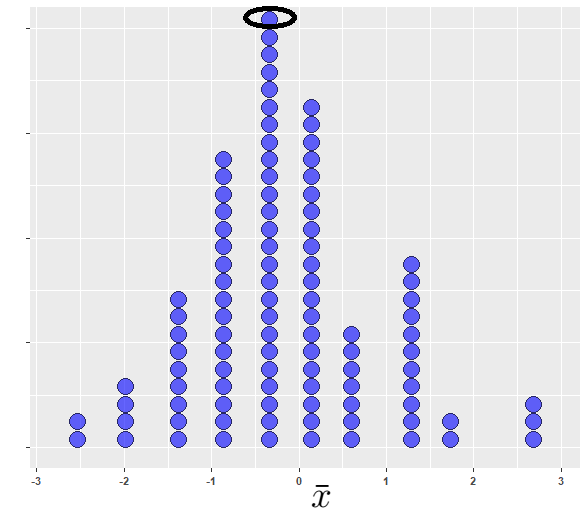
\includegraphics[scale=0.5]{100SamplesSize25FromN0_5}
      \caption{The sampling distribution of $\bar{x}$ of 100 samples with size 25}
      \label{100SamplesSize25FromN0_5}
   \end{figure}
   
   \begin{textblock}{4.2}(14, -5)
   \textblockcolor{dollarbill}
    \noindent Is the distribution of the sample data in table \ref{OneSampleSize25} the same as the sampling distribution in figure \ref{100SamplesSize25FromN0_5}?
   \end{textblock}
       \noindent \colorbox{babypink}{\parbox{\textwidth}{
     Distinguish \textbf{the sampling distribution}, \textbf{the distribution of the sample data} and \textbf{the population distribution}.
          }}\vspace{0.3cm}\\
     
    \noindent Draw simple random samples with sample size 20 from a population with 50 black balls and 150 white balls. The statistics of the proportion of black balls in the samples is denoted $\hat{p}$. Figure \ref{SamplingDsitributionPHat} gives the sampling distribution $\hat{p}$ of 100 such samples.
      \begin{figure}[H]
         \centering
         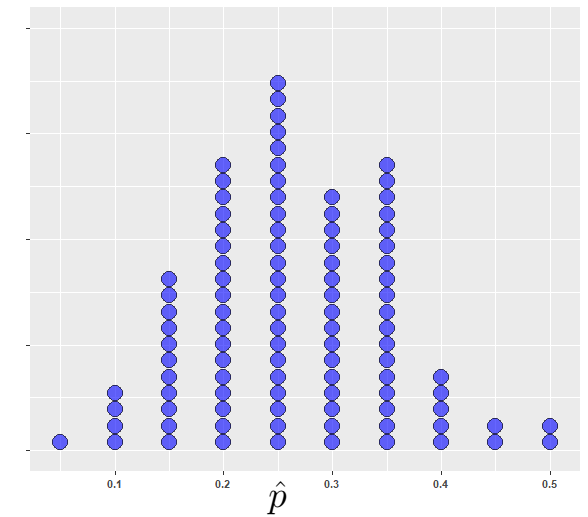
\includegraphics[scale=0.4]{SamplingDsitributionPHat}
         \caption{Sampling distribution of $\hat{p}$}
         \label{SamplingDsitributionPHat}
     \end{figure} 
     \newpage
  \noindent \textbf{Unbiased estimator}\vspace{0.3cm}\\
  A statistic is a random variable used to estimate the corresponding parameter and sometimes this statistic is called an \textbf{estimator} of the parameter. In the following, we will use \textit{estimator} and \textit{statistic} interchangeablely.\vspace{0.3cm}\\
  \noindent Each value of this estimator is an \textbf{estimate}. If the mean(expected value) of the this estimator equals the parameter to be estimated, it is an \textbf{unbiased estimator}.\vspace{0.3cm}\\
  $\reallywidehat{p}, \overline{x}, s_X^2$ are unbiased estimators of $p, \mu, \sigma^2$, which means 
  $$\mu_{\reallywidehat{p}} = p, \qquad
  \mu_{\overline{x}} = \mu, \qquad
  \mu_{s_X^2} = \sigma^2.$$
  Take a look at figure \ref{100SamplesSize25FromN0_5} and figure \ref{SamplingDsitributionPHat}, the center of the sampling distribution is approximately around the parameter to be estimated.\vspace{0.5cm}\\
  
 \noindent \textbf{Variability of a statistic}\vspace{0.3cm}\\ 
 \noindent When a statistic is used to estimate a parameter, we expect it is an unbiased estimator, that is the center of the sampling distribution equal the parameter and the estimation is \textit{accurate}. We also expect the sampling distribution of the statistic  is small, in this way the estimation is more \textit{precise} \vspace{0.3cm}\\
If the sample is more representative of the population, the estimates are more close to the parameter, the variability of the estimator is smaller. Previously, we learned \textit{stratified random sample} is more representative than SRS, and the sampling distribution of those samples has a smaller variability. The other way to make a sample more representative is to increase sample size. The larger the sample size the smaller the variability of the sampling distribution of the statistics. Latter we will learn how to quantify the relationship between the sample size and the variability of the distribution of the statistics. But, we need to know one fact now:\vspace{0.3cm}\\

   
   \noindent \colorbox{babypink}{\parbox{\textwidth}{
    The \textbf{variability of a statistic} is described by the spread of its sampling distribution.  Larger samples give smaller spreads. The spread of the sampling distribution does not depend much on the size of the population, as long as the population is at least 10 times larger than the sample.
    }}\vspace{0.3cm}\\
    
  \noindent  In figure \ref{VariabilityAndBias} take the bull's\textendash eys as the parameter to be estimated.
    
    \begin{figure}[H]
         \centering
         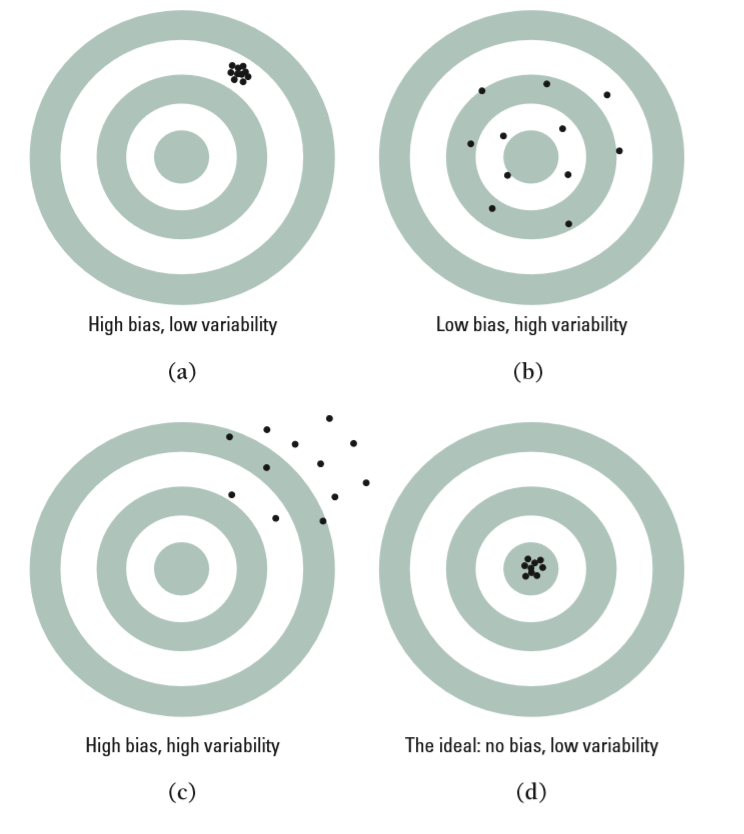
\includegraphics[scale=0.4]{VariabilityAndBias}
         \caption{Illustration of the variability and bias}
         \label{VariabilityAndBias}
    \end{figure}
\newpage

\noindent \colorbox{champagne}{\parbox{\textwidth}{
\textbf{Doing Homework!}\vspace{0.3cm}\\
 A school newspaper article claims that 60\% of the students at a large high school did all their assigned homework last week. Some skeptical AP\textsuperscript{\textregistered} Statistics students want to investigate whether this claim is true, so they choose an SRS of 100 students from the school to interview. What values of the sample proportion $\reallywidehat{p}$ would be consistent with the claim that the population proportion of students who completed all their homework is $p=0.6$?  To find out, we used Fathom software to simulate choosing 250 SRSs of size $n = 100$ students from a population in which $p = 0.60$. The figure below is a dotplot of the sample proportion $\reallywidehat{p}$ of students who did their homework.
 \begin{figure}[H]
     \centering
     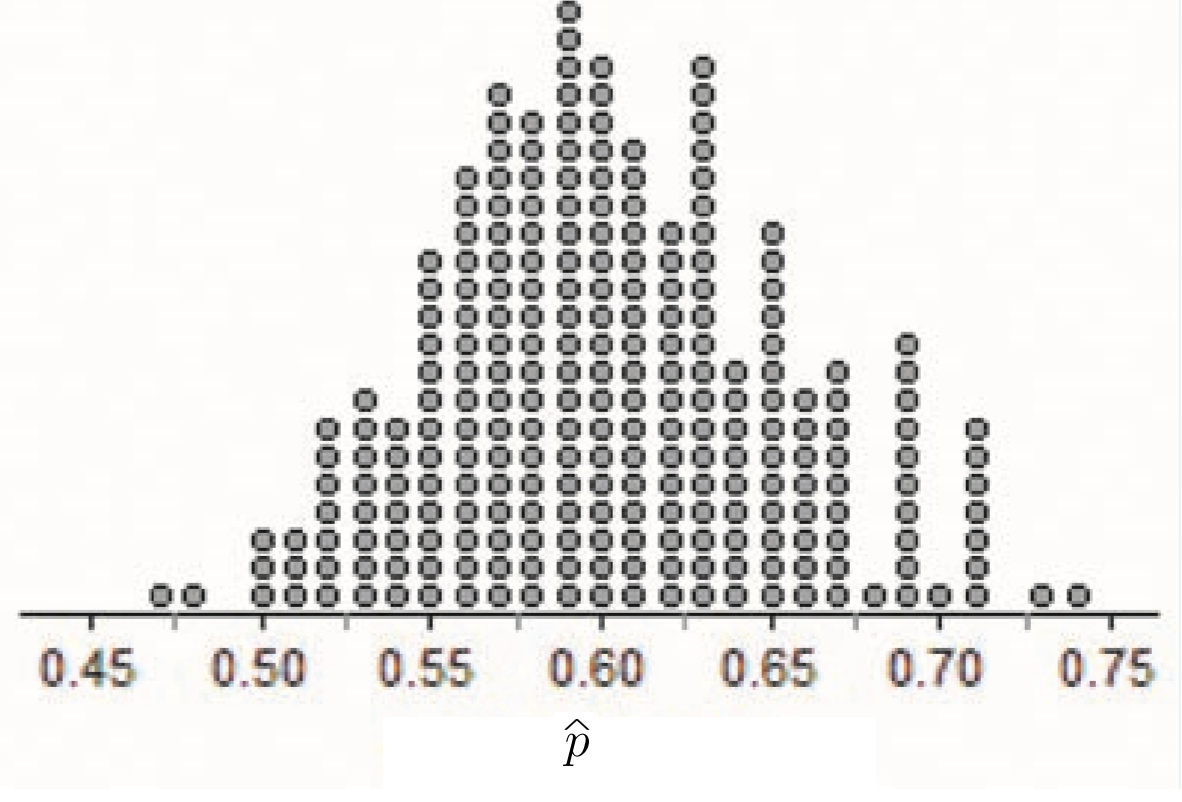
\includegraphics[scale=0.3]{DoingHomework}
 \end{figure}
    \begin{enumerate}[(a)]
        \item There is one dot on the graph at 0.73. Explain what this value represents.
        \item Describe the distribution. Are there any obvious outliers?
        \item  Would it be surprising to get a sample proportion of 0.45 or lower in an SRS of size 100 when $p = 0.6$ ? Justify your answer.
        \item  Suppose that 45 of the 100 students in the actual sample say that they did all their homework last week. What would you conclude about the newspaper article’s claim? Explain.
    \end{enumerate}
}}
\newpage

\section{Sampling distribution of $\hat{p}$}
Suppose there are $N$ balls, the proportion of black balls is $p$, and the others are white balls. Pick an SRS of size $n$(without replacement), and the proportion of black balls in this sample is $\displaystyle{\reallywidehat{p} = \frac{X}{n}}$, where $X$ is the number of black balls in the sample. Let's find out the sampling distribution of the statistic $\reallywidehat{p}$.
    \begin{enumerate}[(1)]
        \item \textbf{Use classical probability model to calculate} $\textbf{P}(\reallywidehat{p} = r)$.\vspace{0.3cm}\\
        The number of all possible outcomes with $\reallywidehat{p} = r$ is given by 
        $${}_{nr}\textbf{C}_{Np}\times {}_{n(-r)}\textbf{C}_N(1-p).$$
        The number of all possible outcomes is given by: ${}_n\textbf{C}_N$\vspace{0.3cm}\\
        $$\textbf{P}(\reallywidehat{p} = r) = \frac{{}_{nr}\textbf{C}_{Np}\times {}_{n(-r)}\textbf{C}_N(1-p)}{{}_n\textbf{C}_N}$$
        \begin{textblock}{3}(-3, -4)
        \textblockcolor{dollarbill}
        Can you make a simple deduction about the results  on the right?
        \end{textblock}
        
        \item \textbf{Use binomial distribution to calculate}$\textbf{P}(\reallywidehat{p} = r)$.\vspace{0.3cm}\\
        Suppose $n \leq 10\%\,N$, the \textbf{10 \% condition} is met. The outcome for the individuals in the sample are approximately independent with each other. $X$ is approximately $\textbf{B}(n, n\reallywidehat{p})$\vspace{0.3cm}\\
        $$\textbf{P}(\reallywidehat{p}) = {}_{nr}\textbf{C}_n\,p^{nr}\,(1-p)^{n-nr}$$
        \item \textbf{Use Normal distribution}\vspace{0.3cm}\\
        In addition to the \textbf{10\% condition}, the \textbf{large counts condition} is met($np \leq 10, \qquad n(1-p) \leq 10$). Then X is approximately normal. 
        $$X \sim \textbf{N}(\mu_X, \sigma_X), \qquad \mu_X = np,\quad \sigma_X = \sqrt{np(1-p)}$$
        
        \begin{textblock}{3.6}(-3.5, 2)
           \textblockcolor{dollarbill}
           What conditions must be met in order to use the formulas for $\mu_{\reallywidehat{p}}$ and $\sigma_{\reallywidehat{p}}$ ?
        \end{textblock}
        
        
        $\displaystyle{\reallywidehat{p} = \frac{X}{n}}$ is normally distributed according to the knowledge of \textit{transforming random variables}, $\reallywidehat{p} \sim N(\mu_{\reallywidehat{p}}, \sigma_{\reallywidehat{p}})$. The $\mu_{\reallywidehat{p}}$ and  $\sigma_{\reallywidehat{p}}$ are given bellow.
        $$\mu_{\reallywidehat{p}} = \frac{1}{n}\mu_X = p$$
        $$\sigma_{\reallywidehat{p}} = \frac{1}{n}\sigma_X = \sqrt{\frac{p(1-p)}{n}}$$       
    \end{enumerate}
    
\colorbox{babypink}{\parbox{\textwidth}{
 From the above equations we can come up with two conclusions
 \begin{enumerate}[\Roman*.]
     \item $\reallywidehat{p}$ is an unbiased estimator of $p$.
     \item If the sample size increases by timing  factor $C$, the standard deviation of $\reallywidehat{p}$ decreases by timing factor $\displaystyle{\frac{1}{\sqrt{C}}}$.
 \end{enumerate}
 \begin{textblock}{3}(-3.5, -3)
 Explain why we can come up with those two conclusions?
 \end{textblock}
}}
\newpage

\colorbox{champagne}{\parbox{\textwidth}{
\textbf{Do you go to church?}\vspace{0.3cm}\\
 The Gallup Poll asked a random sample of 1785 adults whether they attended church during the past week. Let $\reallywidehat{p}$ be the proportion of people in the sample who attended church.  A newspaper report claims that 40\% of all U.S. adults went to church last week. Suppose this claim is true.\vspace{0.3cm}\\
    \begin{enumerate}[(a)]
        \item What is the mean of the sampling distribution of $\reallywidehat{p}$. Why?
        \item Find the standard deviation of the sampling distribution of $\reallywidehat{p}$. Check to see if the 10\% condition is met.
        \item Is the sampling distribution of $\reallywidehat{p}$ approximately normal? Check to see if the large counts condition is met?
        \item Of the respondents, 44\% said they did attend church last week. Find the probability of obtaining a sample of 1785 adults in which 44\% or more say they attended church last week if the newspaper report's claim is true. Dose this poll give convincing evidence against the claim? Explain.
    \end{enumerate}     
}}
     \newpage
     
 \section{The sampling distribution of $\mathbf{\bar{x}}$}
  Choose an SRS of size $n$ from a population of size $N$, and variable $X_i$ is the measurement on the $i$th individual in the sample.
    \begin{enumerate}[(1)]
        \item \textbf{Suppose the population is normally distributed} $N(\mu, \sigma)$.
        $$X_i \sim N(\mu, \sigma), \quad \mu_{X_i} = \mu, \quad \sigma_{X_i} = \sigma, \qquad i = 1, 2, \cdots, n.$$
        $$\text{sample mean:}\quad\overline{x} = \frac{1}{n}\, (X_1 + X_2 + \cdots + X_n) = \frac{1}{n}\sum_{i=1}^n X_i$$
        $$\mu_{\overline{x}} = \frac{1}{n}\, \sum_{i=1}^n \mu  = \mu$$
        \vspace{0.3cm}
        \begin{enumerate}[$\bullet$]        
        \item \textbf{ If 10\% condition} ($\mathbf{n \leq 10\%\,N}$) \textbf{is met}.
                $$\textbf{Var}(\overline{x}) = (\frac{1}{n})^2 \,\,\textbf{Var}(\sum_{i=1}^n X_i) = (\frac{1}{n})^2 \,\, \sum_{i=1}^n \textbf{Var}(X_i) = \frac{\sigma^2}{n}$$
        $$\sigma_{\overline{x}} = \sqrt{\textbf{Var}(\overline{x})} = \frac{\sigma}{\sqrt{n}}$$ 
         \end{enumerate}
         
         \begin{textblock}{4}(-3.5, -4)
         \textblockcolor{dollarbill}
         Why the \textbf{10\% condition} is required for the formula  of $\sigma_{\overline{x}}$ here?\vspace{0.2cm}\\         
         Is the \textbf{10\% condition} required for the formula of $\mu_{\overline{x}}?$
         \end{textblock}
         \vspace{0.8cm}
         
         If the \textbf{10\% condition} ($\mathbf{n \leq 10\%\,N}$) is met and the population is normally distributed, then, according to the knowledge of "combination of independent normal random variables" in \textit{chapter 5}, $\overline{x}$ is normally distributed.
         $$\overline{x} \sim N(\mu_{\overline{x}}, \sigma_{\overline{x}})$$
The $\mu_{\overline{x}}$ and $\sigma_{\overline{x}}$ are given by the above formulas.\vspace{0.6cm}

\item \textbf{Don't know whether the population distribution is normal or not}.\vspace{0.3cm}\\
The sampling distribution of a statistic is closely related to the sampling distribution. However in the case of sample distribution, there is a very important and elegant theorem, called \textbf{central limit theorem(CLT)}, which guarantees the sampling distribution of sample mean $\overline{x}$ is approximately normal as the sample size $n$ increases. Let's take a look at some simulations.\vspace{0.3cm}\\     

    We will sample from a population with probability density function 
    $$f(x) = e^{-x}  \qquad x \in [0, +\infty).$$
    The density curve of this distribution is strongly right skewed as shown by figure \ref{GammaDistribution}. 
    
        \begin{figure}[H]
         \centering
         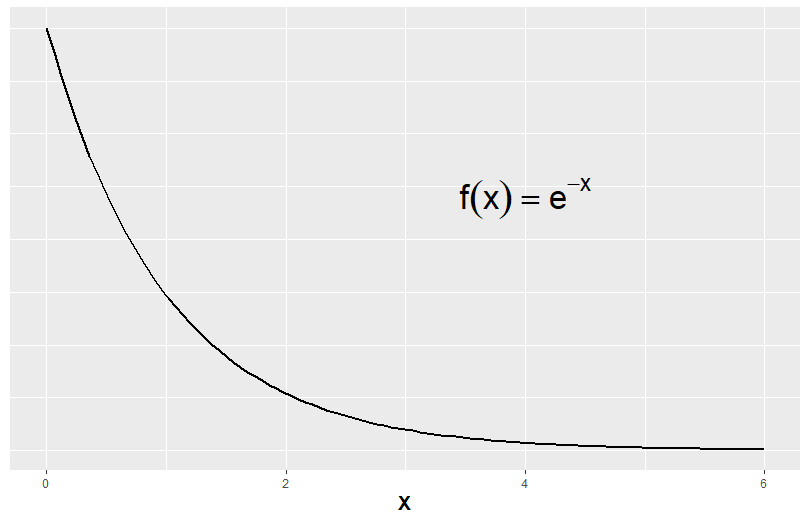
\includegraphics[scale=0.3]{GammaDistribution}
         \caption{A strongly right\textendash skewed distribution}
         \label{GammaDistribution}
        \end{figure}
  
    
   Figure \ref{CLT} shows the sampling distribution of $\overline{x}$ of 500 samples of different sample sizes: $n = 5, 10, 20, 40, 80, 160$. We can tell that the distribution become more and more symmetric. If you pay attention to the range of the distribution, which is a measurement of the variability of the sampling distribution of $\overline{x}$, you will find the range decreases as the sample size increase. This verifies what we learned before about the relationship between sample size and variability.

   \begin{figure}[H]
       \centering
       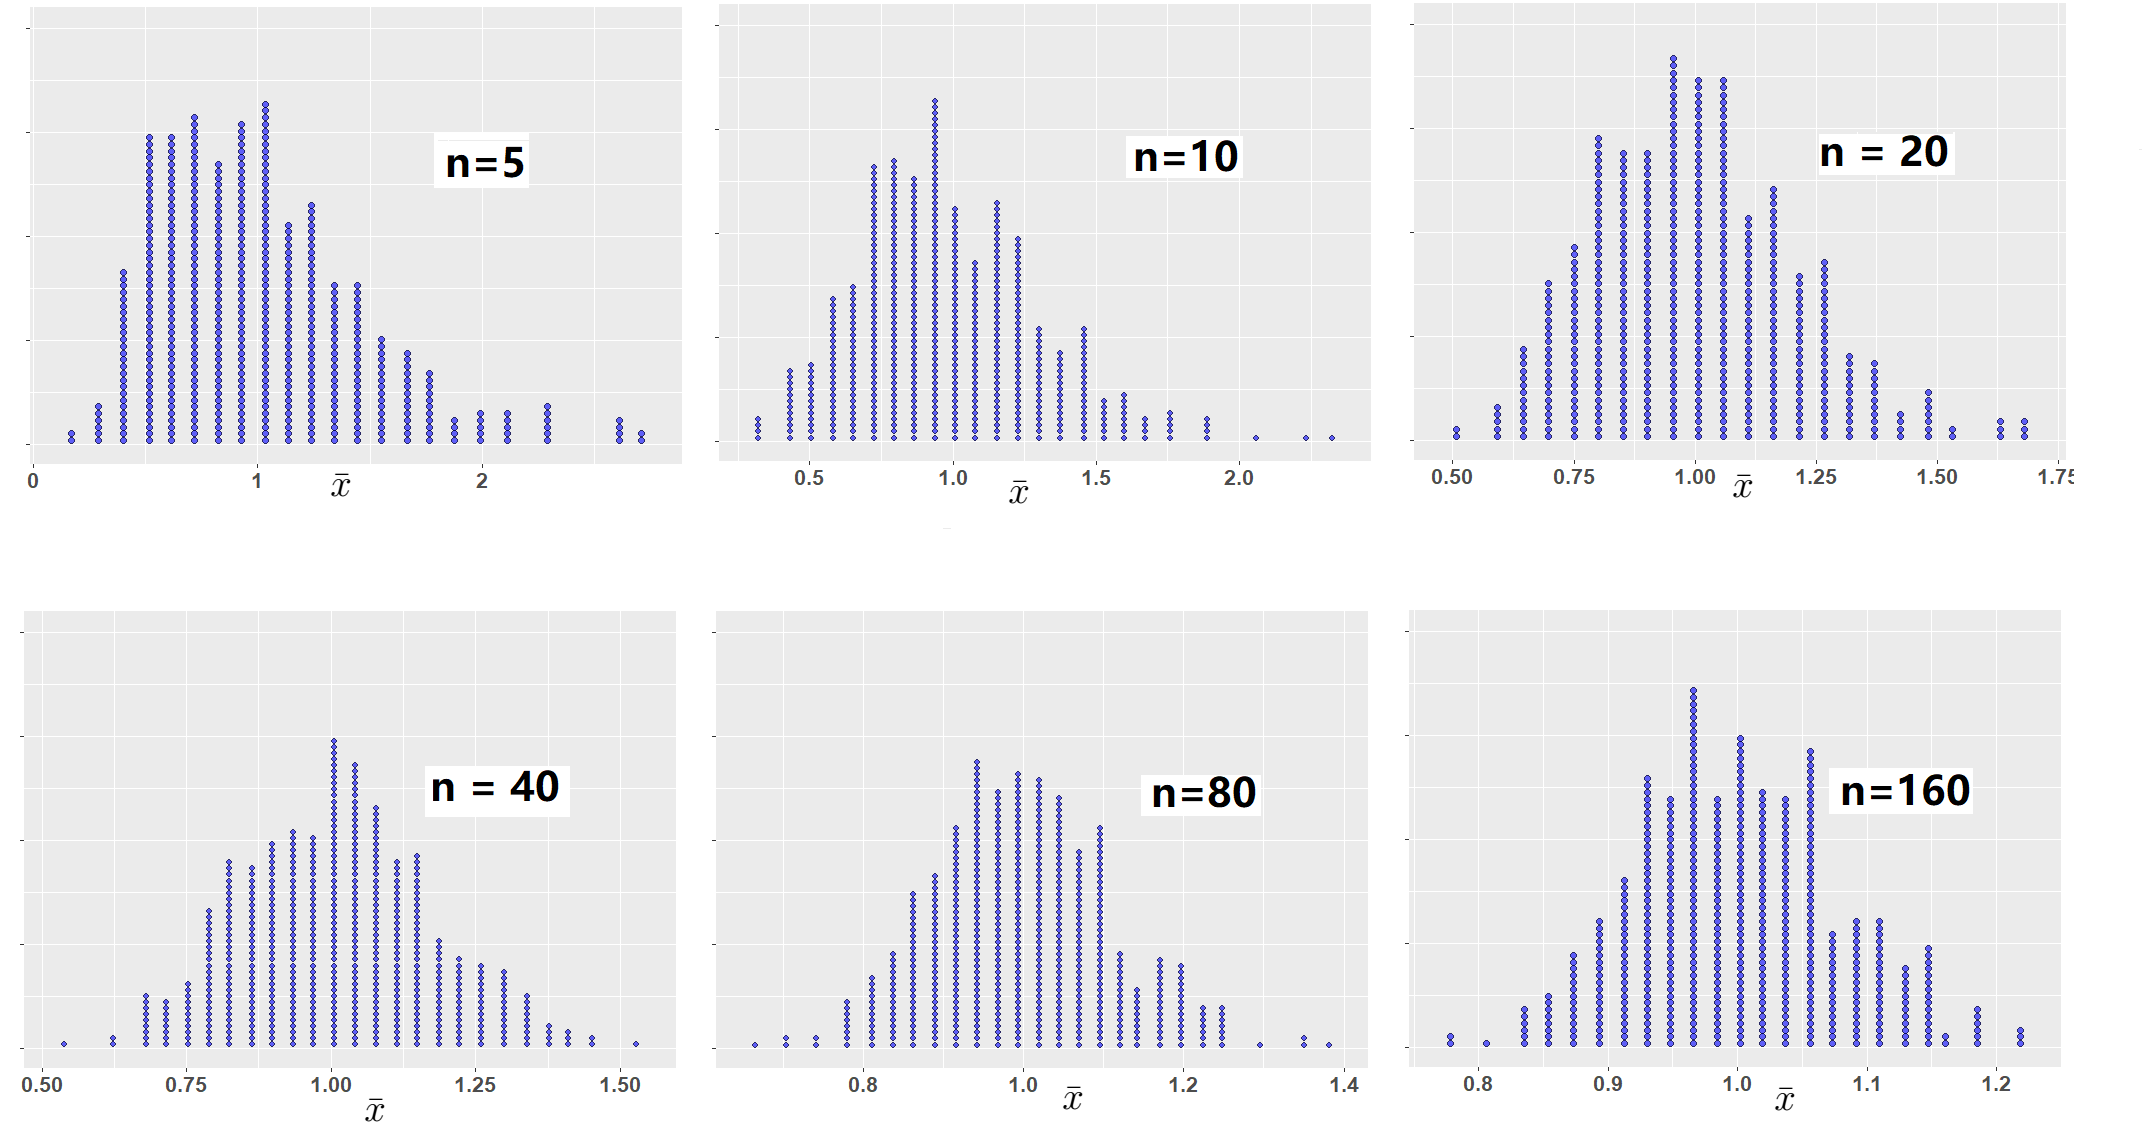
\includegraphics[scale=0.45]{CLT}
       \caption{Demonstration of \textbf{Central Limit Theorem(CLT)}}
       \label{CLT}
   \end{figure}

    \colorbox{babypink}{\parbox{\textwidth}{
    \textbf{Central Limit Theorem(CLT)}\vspace{0.3cm}\\
    Draw an SRS of size n from any population with mean $\mu$ and finite standard deviation $\sigma$. The \textbf{central limit theorem (CLT)}says that when $n$ is large, the sampling distribution of the sample mean $\overline{x}$ is approximately Normal, $N(\mu, \frac{\sigma}{\sqrt{n}})$.\vspace{0.3cm}\\
    As a rule of thumb, if $\mathbf{n\geq 30}$, $n$ is large enough invoke \textbf{CTL}.
    }}
    \newpage
    
    \item \textbf{The t-distribution}\vspace{0.3cm}
 
  \hspace{-1cm}\colorbox{babypink}{\parbox{\textwidth}{
  Previously we learned that if the \textbf{10\% condition}($n \leq 10\%\, N$) is met and  either \textbf{(1) the population is normally distributed}, or  (2) \textbf{the sample is a large sample} ($\mathbf{n \geq 30}$), then the sampling distribution of $\overline{x}$ is approximately normal. 
  $$\overline{x} \sim N(\mu_{\overline{x}}, \sigma_{\overline{x}})
  , \qquad \mu_{\overline{x}} = \mu, \quad \sigma_{\overline{x}} = \frac{\sigma}{\sqrt{n}},$$
 where $\mu$ and $\sigma$ are population mean and population standard deviation.
  }}\vspace{0.3cm}\\
\textbf{What if the population standard deviation $\mathbf{\sigma}$ is unknown?} In this case, the sampling distribution can be described by \textbf{t-distribution}.\vspace{0.6cm}\\
If $\overline{x}\sim \displaystyle{N(\mu, \frac{\sigma}{\sqrt{n}})}$, then $\displaystyle{t = \frac{\overline{x}-\mu}{s_X/\sqrt{n}}}$ follows a \textbf{t-distribution} with $\textbf{df} = n-1$, where \textbf{df} is the \textbf{degree of freedom}.

    \begin{textblock}{3.5}(-3.5, -2)
    \textblockcolor{dollarbill}
    What is the distribution of $$z = \frac{\overline{x}-\mu}{s_X/\sqrt{n}}$$
    \end{textblock}

    \begin{figure}[H]
        \centering
        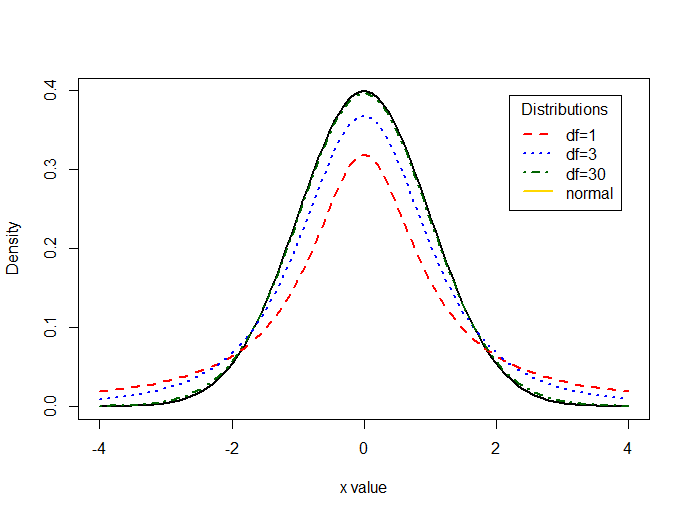
\includegraphics[scale=0.6]{TDdistributionsNormalDistribution}
        \caption{t\textendash distributions and Normal distribution}
        \label{TDdistributionsNormalDistribution}
    \end{figure}
 Figure \ref{TDdistributionsNormalDistribution}, gives t-distributions with different degree of freedom and standard normal distribution.  we can have the following statements by reading this figure.
    \begin{itemize}
        \item The t-distribution is symmetric with center 0
        \item The t-distribution has a larger variance than $N(0, 1)$
        \item The larger the degree of freedom(\textbf{df}), the smaller the variance of the t-distribution.
        \item As \textbf{df} increases, the a-distribution approximates to standard normal distribution $N(0, 1).$ 
    \end{itemize}  
    \end{enumerate}  
    \newpage
    
    \colorbox{champagne}{\parbox{\textwidth}{
    \textbf{The Principal's Suspicion}\vspace{0.3cm}\\
    A report claims that the height of high school kids follows a Normal distribution with mean $\mu = 168\, \text{cm}$ and standard deviation $\sigma = 9\, \text{cm}$. A high school principal suspect that the average height of the students in this school is higher. In order to test the principal's suspicion, an SRS of 9 students were drawn.\vspace{0.3cm}\\
    Assume the report's claim is true. Solving the following problems. 
    \begin{enumerate}[(a)]
       \item  Find the probability that a randomly selected young woman is taller than $175\, \text{cm}$. Show your work.
       \item Find the probability that the mean height of the SRS  exceeds $175\, \text{cm}$. Show your work.
       \item  The heights of the 9 students in the SRS are given below, in centemeters.
$$172\quad178\quad168\quad183\quad180\quad165\quad175\quad177\quad170\quad$$
Find the statistic $t$ of this sample.
   \item If the population standard deviation($\sigma = 9\, \text{cm}$) is unknown. Find the probability that a randomly chosen SRS of size 9 with $t$ larger than the value in the proceeding problem.
   \item What can you say about the principal's suspicion.
    \end{enumerate}
    }} 
    \newpage
    \noindent\colorbox{champagne}{\parbox{\textwidth}{
    \textbf{Are We Richer?}\vspace{0.3cm}\\
   The yearly income of Chinese people is strongly right-skewed. According to the report from the government, the average yearly income of Chinese people is $74,318$ \textyen \hspace{3pt}  and the standard deviation of the income of the nation is $30,000$ \textyen \hspace{3pt} in 2017. \vspace{0.3cm}\\
   The leader of a province thought people in this province might be richer. In order to test this though,  an SRS of size 100 is drawn, with sample mean $ 77,000$ \textyen \hspace{3pt}and the standard deviation  $40, 000$\textyen \hspace{3pt}.\vspace{0.3cm}\\
   Answer the following questions while assuming the report from the government is true for this province as well.
   \begin{enumerate}[(a)]
       \item Find the probability a randomly chosen person with a yearly income 77,000 \textyen \hspace{3pt} or higher?
       \item Find the probability a randomly chosen SRS with sample mean 
        77,000 \textyen \hspace{3pt} or higher?
        \item Suppose the population standard deviation is unknown and and the standard deviation of the sample is  $40, 000$\textyen \hspace{3pt}.\vspace{0.3cm}, find the $t$ value of this sample.
        \item Find the probability that a randomly chosen SRS of size 100 has $t$ value larger than the value in previous problem.
        \item Do you think people are richer in this province according to the result in (d)?        
   \end{enumerate}
    }} \newpage                                   
\end{document}